% 2.5D complete heat path (TikZ): die ->(ubump)-> interposer ->(C4)->
% substrate ->(PCB)-> ambient, plus the heatsink branch die ->(TIM)->
% heatsink ->(convection)-> ambient. Both cooling paths coexist; the two
% branches use different colors (amber = heatsink branch, blue = substrate
% branch). Physical layers (ubump/C4/TIM) are labeled as chain segments;
% every branch carries its physical path type + value provenance; nodes
% carry role/size. All routing orthogonal; sans-serif.
%
% Sources: config/thermal/*.yaml values (r_vert lumped = 1.5 K/W,
% r_tim = 0.3 K/W, h*A -> R_conv = 0.69 K/W) + thermal-module-catalog
% formulas for the per-segment decomposition (t/(kA)); per-segment
% numeric values come from config/params or literature, not fabricated.
\documentclass[border=10pt]{standalone}
\usepackage{sfmath}
\renewcommand{\familydefault}{\sfdefault}
\usepackage{tikz}
\usetikzlibrary{arrows.meta, shapes.geometric}
\definecolor{diefill}{HTML}{E8F0FE}
\definecolor{dieedge}{HTML}{1A73E8}
\definecolor{ipfill}{HTML}{F3E8FD}   % interposer: light purple
\definecolor{ipedge}{HTML}{9334E6}
\definecolor{subfill}{HTML}{FFF4E5}  % substrate: light amber
\definecolor{subedge}{HTML}{B45309}
\definecolor{pcbfill}{HTML}{E6F4EA}  % PCB: light green
\definecolor{pcbedge}{HTML}{188038}
\definecolor{hsfill}{HTML}{E0F2F1}   % heatsink: teal rounded rect
\definecolor{hsedge}{HTML}{00695C}
\definecolor{bndfill}{HTML}{F1F3F4}
\definecolor{bndedge}{HTML}{5F6368}
\definecolor{segsub}{HTML}{1A73E8}   % substrate-path segments: blue
\definecolor{seghs}{HTML}{B45309}    % heatsink-path segments: amber
\begin{document}
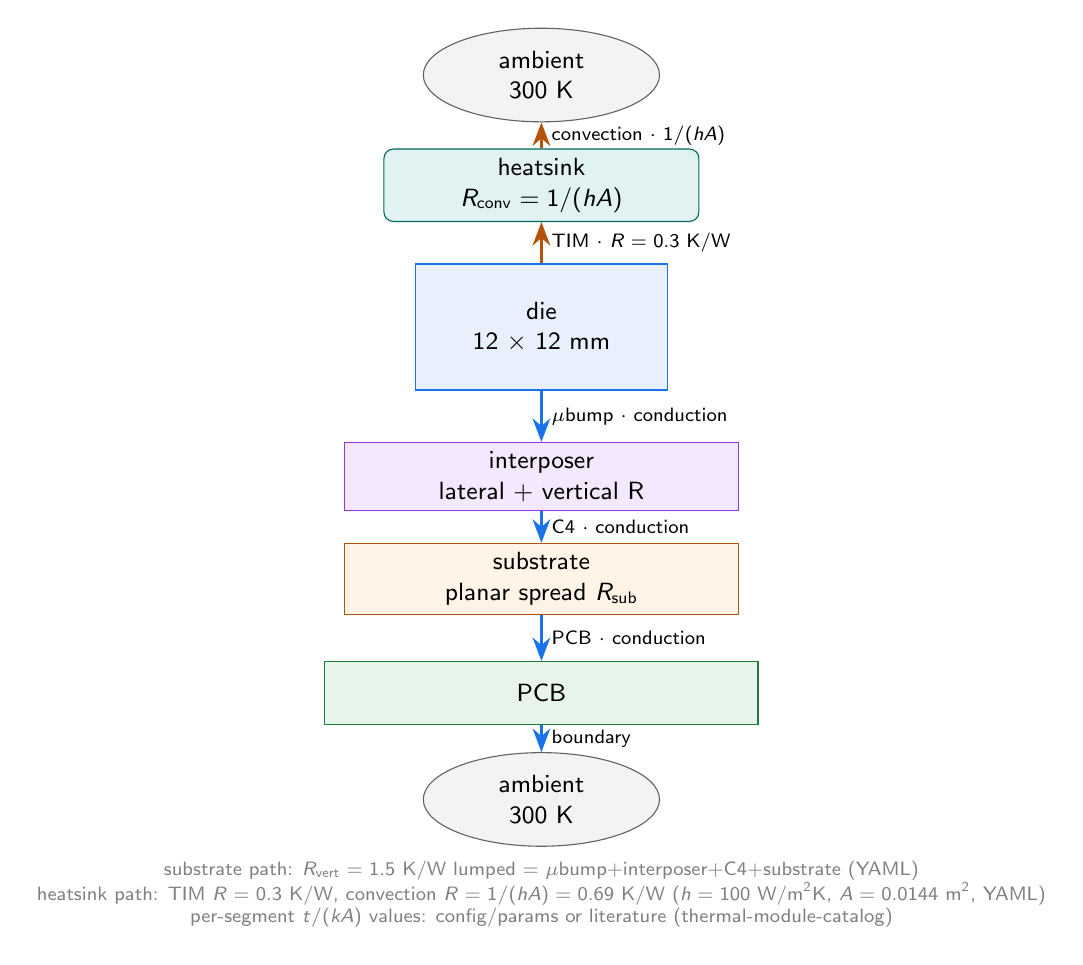
\begin{tikzpicture}[
  die/.style={rectangle, draw=dieedge, fill=diefill, minimum width=3.2cm,
              minimum height=1.6cm, align=center, font=\small},
  layer/.style 2 args={rectangle, draw=#1, fill=#2, minimum width=5.0cm,
              minimum height=0.8cm, align=center, font=\small},
  hs/.style={rectangle, rounded corners=0.12cm, draw=hsedge, fill=hsfill,
             minimum width=4.0cm, minimum height=0.8cm, align=center, font=\small},
  bnd/.style={ellipse, draw=bndedge, fill=bndfill, minimum width=3.0cm,
              minimum height=1.0cm, align=center, font=\small},
  segsub/.style={draw=segsub, thick, -{Stealth[length=3mm]}, rounded corners=0.08cm},
  seghs/.style={draw=seghs, thick, -{Stealth[length=3mm]}, rounded corners=0.08cm},
  lab/.style={font=\scriptsize},
]
% ---- substrate cooling path (blue): die -> ubump -> interposer -> C4 -> substrate -> PCB -> ambient
\node[die] (die) at (0, 1.5) {die\\12 $\times$ 12 mm};
\node[layer={ipedge}{ipfill}] (interposer) at (0, -0.4) {interposer\\lateral + vertical R};
\node[layer={subedge}{subfill}] (substrate) at (0, -1.7) {substrate\\planar spread $R_{\mathrm{sub}}$};
\node[layer={pcbedge}{pcbfill}, minimum width=5.5cm] (pcb) at (0, -3.15) {PCB};
\node[bnd] (ambient) at (0, -4.5) {ambient\\300 K};
\draw[segsub] (die.south) -- node[right, lab] {$\mu$bump $\cdot$ conduction} (interposer.north);
\draw[segsub] (interposer.south) -- node[right, lab] {C4 $\cdot$ conduction} (substrate.north);
\draw[segsub] (substrate.south) -- node[right, lab] {PCB $\cdot$ conduction} (pcb.north);
\draw[segsub] (pcb.south) -- node[right, lab] {boundary} (ambient.north);
% ---- heatsink branch (amber): die -> TIM -> heatsink -> convection -> ambient
\node[hs] (heatsink) at (0, 3.3) {heatsink\\$R_{\mathrm{conv}}=1/(hA)$};
\node[bnd] (ambient_hs) at (0, 4.7) {ambient\\300 K};
\draw[seghs] (die.north) -- node[right, lab] {TIM $\cdot$ $R=0.3$ K/W} (heatsink.south);
\draw[seghs] (heatsink.north) -- node[right, lab] {convection $\cdot$ $1/(hA)$} (ambient_hs.south);
% branch annotation: physical path type + value provenance (3 lines)
\node[lab, align=center, text=gray] at (0, -5.7) {
  substrate path: $R_{\mathrm{vert}}=1.5$ K/W lumped $= \mu$bump+interposer+C4+substrate (YAML)\\
  heatsink path: TIM $R=0.3$ K/W, convection $R=1/(hA)=0.69$ K/W ($h=100$ W/m$^2$K, $A=0.0144$ m$^2$, YAML)\\
  per-segment $t/(kA)$ values: config/params or literature (thermal-module-catalog)};
\end{tikzpicture}
\end{document}
